\documentclass{article}

% ================== Packages ==================
\usepackage{tikz}
\usepackage{quantikz}
\usepackage{braket}
\usepackage[margin=1in]{geometry}
\usepackage{enumitem}
\usepackage{float}
\usepackage{amsmath}

\allowdisplaybreaks

% ================== Title ==================
\title{Introduction to Quantum Information and Quantum Computing\\Assignment 1}
\author{Manuel Santos -- 2019231352}
\date{November 2025}

\begin{document}

\maketitle

% ================== Introduction ==================
\section*{Introduction}
This report presents the solution to Assignment 1 of the Introduction to Quantum Information and Quantum Computing course.

The goal of this assignment is to illustrate a fundamental feature of quantum mechanics: measurement outcomes do not, in general, possess predetermined values prior to measurement—unless one is willing to accept the possibility of faster-than-light communication.

% ================== 1 ==================
\section{Preparation of a shared state}

Alice (A), Bob (B), and Charlie (C) are separated from each other by a considerable distance. A source (S) prepares three qubits in the so-called $\ket{\mathrm{GHZ}}$ state, according to the circuit below, and sends one qubit to each of them. As always, the qubits start in the state
\[
\ket{000}\quad (\ket{\mathrm{CBA}}\ \text{ordering})
\]
before passing through the circuit.

\begin{figure}[H]
    \centering
    \begin{minipage}{0.49\textwidth}
        \centering
        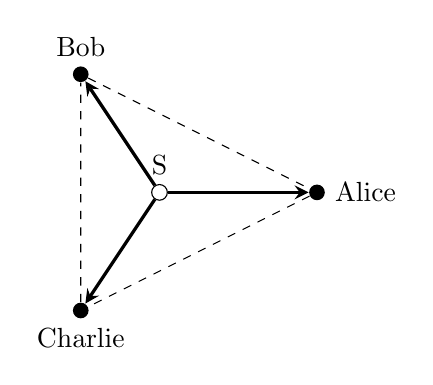
\begin{tikzpicture}[>=stealth, node distance=2cm]
            \node[fill=black, circle, inner sep=2pt, label=above:{Bob}] (bob) at (0,3) {};
            \node[fill=black, circle, inner sep=2pt, label=right:{Alice}] (alice) at (3,1.5) {};
            \node[fill=black, circle, inner sep=2pt, label=below:{Charlie}] (charlie) at (0,0) {};
            \node[draw, circle, inner sep=2pt, label=above:{S}] (s) at (1,1.5) {};
            \draw[dashed] (bob) -- (alice) -- (charlie) -- (bob);
            \draw[->, line width=1.2pt] (s) -- (bob);
            \draw[->, line width=1.2pt] (s) -- (charlie);
            \draw[->, line width=1.2pt] (s) -- (alice);
        \end{tikzpicture}
    \end{minipage}
    \begin{minipage}{0.49\textwidth}
        \centering
        \begin{quantikz}
            \lstick{$A:$} & \gate{H} & \slice[style=black]{$\ket{\mathrm{Barrier}}$} & & \ctrl{1} & & \ctrl{2} & & \slice[style=black]{$\ket{\mathrm{GHZ}}$} & & \\
            \lstick{$B:$} &          &                                              & & \targ{}  & &           & & & & \\
            \lstick{$C:$} &          &                                              & &          & & \targ{}  & & & &
        \end{quantikz}
    \end{minipage}
    \caption{System layout and quantum circuit preparing the GHZ state}
    \label{fig:ex1_system}
\end{figure}

\begin{enumerate}[label=(\alph*)]
    \item
    \begin{enumerate}[label=\roman*)]
        \item
        Let $\ket{\mathrm{Barrier}}$ denote the state at the first barrier. Since the Hadamard gate is applied only to qubit $A$ (the least significant qubit in the $\ket{\mathrm{CBA}}$ ordering), we obtain
        \[
        \ket{000}
        \xrightarrow{\mathrm{H}_A}
        \ket{00}\!\left(\frac{\ket{0}+\ket{1}}{\sqrt{2}}\right)
        =
        \frac{1}{\sqrt{2}}\ket{000}
        +
        \frac{1}{\sqrt{2}}\ket{001}
        = \ket{\mathrm{Barrier}}.
        \]

        \item
        Starting from $\ket{\mathrm{Barrier}}$, we apply a CNOT gate with $A$ as control and $B$ as target, followed by a CNOT with $A$ as control and $C$ as target:
        \[
        \ket{\mathrm{Barrier}}
        \xrightarrow{\mathrm{CNOT}_{A,B}}
        \frac{1}{\sqrt{2}}\ket{000}
        +
        \frac{1}{\sqrt{2}}\ket{011}
        \xrightarrow{\mathrm{CNOT}_{A,C}}
        \frac{1}{\sqrt{2}}\ket{000}
        +
        \frac{1}{\sqrt{2}}\ket{111}
        = \ket{\mathrm{GHZ}}.
        \]
    \end{enumerate}

    At the first barrier, the system is in a superposition of $\ket{000}$ and $\ket{001}$. After the CNOT operations, this superposition is extended across all three qubits, producing the maximally entangled GHZ state.

    \item
    Measuring Alice’s qubit collapses the state:
    \begin{itemize}
        \item If Alice measures $0$, Bob and Charlie collapse to $\ket{00}$
        \item If Alice measures $1$, Bob and Charlie collapse to $\ket{11}$
    \end{itemize}
    From Bob’s or Charlie’s local perspective, the outcomes remain random until classical communication occurs.

    \item
    Since $\ket{\mathrm{GHZ}}$ is an equal superposition of $\ket{000}$ and $\ket{111}$, we expect each outcome with probability $1/2$. This behavior is confirmed by simulation, as shown in Figure~\ref{fig:ex1_c}.

    \begin{figure}[H]
        \centering
        \includegraphics[width=0.5\textwidth]{Images/1_c.png}
        \caption{Simulation results for 1024 shots}
        \label{fig:ex1_c}
    \end{figure}
\end{enumerate}

% ================== 2 ==================
\section{Independent Operations}

After receiving their qubits, Alice, Bob, and Charlie independently apply either
\[
M_X = H \quad \text{or} \quad M_Y = HS^\dagger,
\]
followed by measurement.

\begin{enumerate}[label=(\alph*)]
    \item
    When all three apply $M_X$, the resulting state $\ket{\mathrm{XXX}}$ is produced by the circuit in Figure~\ref{fig:mx_circuit}.

    \begin{figure}[H]
        \centering
        \begin{quantikz}[wire types={q,q,q,c}]
            \lstick{$A:$} & \gate{H} & \ctrl{1} & \ctrl{2} & \slice{$\ket{\mathrm{GHZ}}$} & & \gate{H} & & \meter{} & \\
            \lstick{$B:$} &          & \targ{}  &          &                              & & \gate{H} & &          & \meter{} \\
            \lstick{$C:$} &          &          & \targ{}  &                              & & \gate{H} & &          &          \meter{}
        \end{quantikz}
        \caption{Circuit XXX: all parties apply $M_X = H$}
        \label{fig:mx_circuit}
    \end{figure}

    Applying the Hadamard gates yields
    \[
    \ket{\mathrm{XXX}}
    =
    \frac{1}{2}
    \big(
    \ket{000}
    +
    \ket{011}
    +
    \ket{101}
    +
    \ket{110}
    \big).
    \]

    Simulation results are shown in Figure~\ref{fig:ex2_XXX}.

    \begin{figure}[H]
        \centering
        \includegraphics[width=0.5\textwidth]{Images/2_a.png}
        \caption{Simulation results for circuit XXX (1024 shots)}
        \label{fig:ex2_XXX}
    \end{figure}

    \item
    The possible outcomes are $\ket{000}$, $\ket{011}$, $\ket{101}$, and $\ket{110}$. In all cases, the sum $a+b+c$ is even.

    \item
    When exactly one party applies $M_X$ and the others apply $M_Y$, only four outcomes occur, and the sum $a+b+c$ is always odd.

    \item
    The outcomes for each configuration are:
    \begin{itemize}
        \item YYX, YXY, XYY:
        \[
        (C,B,A) = (0,0,1), (0,1,0), (1,0,0), (1,1,1).
        \]
    \end{itemize}
    These results confirm the GHZ correlations.
\end{enumerate}

\end{document}
